\pagebreak
\section{Automatic Generation Control (AGC)}  
Automatic generation control model that calculates RACE and distributes signal to defined controlled generators according to participation factor.
The ACE signal is filtered through a PI before being distributed to each generator through a unique low pass filter that adds the negative of the value to the governor \verb|tg_sig| value.
( NOTE: the \verb|tg_sig| value is equivalent to an addition to the governors $P_{ref}$ value)
The \verb|agc_indx| function creates the required data structures and indices.

%==========================================================================

\subsection{AGC Block Diagram}
The AGC complete process is shown as the three following block diagrams.
RACE and SACE are calculated using PU values assuming B is a positive non-PU value with units of $MW/0.1Hz$
If $K_{bv}$ is not zero, the resulting $RACE$ is not the industry standard $RACE$ value.
The scheduled interchange may be altered by the user via a \verb|mAGC_sig| file that controls the behavior of the $IC_{adj}$ input.

\begin{center}
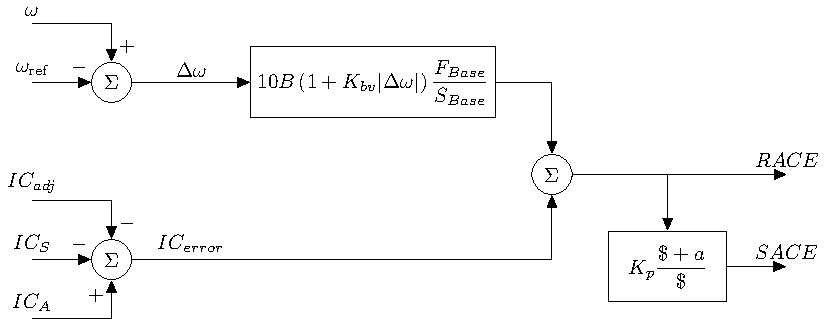
\includegraphics[width=.75\linewidth]{sections/agc/200722-AGCblockdiagram-p1}
\end{center}

$RACE$ and $SACE$ are calculated every time step, however
distribution of $SACE$ is determined by the \verb|startTime| and \verb|actionTime| variables.
Assuming action, the conditional $\Delta\omega$ logic is processed before adjusting the \verb|aceSig| value which is then gained to become \verb|ace2dist|.

\begin{center}
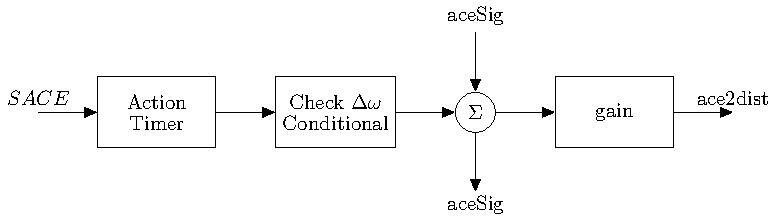
\includegraphics[width=.75\linewidth]{sections/agc/200722-AGCblockdiagram-p2}
\end{center}

The \verb|ace2dist| value is distributed to all controlled generators associated with the AGC model according to their respective participation factor \verb|pF|.
Each \verb|ctrlGen| has a unique low pass filter that processes the signal that is then gained by -1 and added to the existing associated governor \verb|tg_sig| value.

\begin{center}
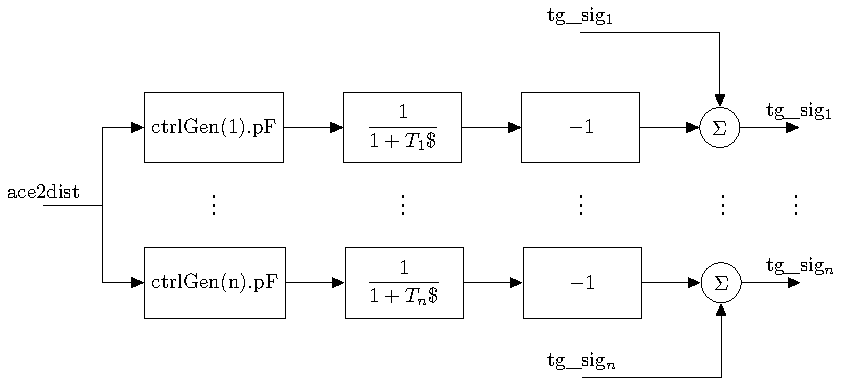
\includegraphics[width=.75\linewidth]{sections/agc/200722-AGCblockdiagram-p3}
\end{center}
% related AGC additions

%==================================================
\subsection{calcAreaVals}  
Calculates total area generation and interchange.
Intentions were to also sum total load, but there were complications with that and work in that direction seemed not entirely useful.

%==========================================================================
\subsection{Weighted Average Frequency (calcAveF)} 
Calculates system and area weighted average frequency.
System values stored in \verb|g.sys.aveF| and area values stored in \verb|g.area.area(x).aveF|.

An average weighted frequency is calculated for the total system and for each area if there are areas detected.
The calculation involves a sum of system inertias that may change with generator trips.
The current algorithm does not account for tripped generators, but was designed to incorporate this feature in the future.

\vspace{1em}
In a system with $N$ generators, $M$ areas, and $N_M$ generators in area $M$, the \verb|calcAveF| function performs the following calculations for each area $M$:

\begin{align*}
%         % calculate weighted average frequency for each area, sum for system
%         runningSysF = 0;
%         runningSysH = 0;
%         for areaN=1:g.area.n_area
%             % calculate area total inertia
%             mNdx = g.area.area(areaN).macBusNdx;
%             g.area.area(areaN).totH(k) = sum(g.mac.mac_con(mNdx,16).*g.mac.mac_con(mNdx,3));
%             % calculate ave weighted f = sum(mac_speed.*MVA.*H) / totH
%             g.area.area(areaN).aveF(k) = sum(g.mac.mac_spd(mNdx,k).*g.mac.mac_con(mNdx,3).*g.mac.mac_con(mNdx,16)) ...
%                 /g.area.area(areaN).totH(k);
%             
%             runningSysF = runningSysF + g.area.area(areaN).aveF(k);
%             runningSysH = runningSysH + g.area.area(areaN).totH(k);
%         end
%         
%         %g.sys.totH(k) = sum(g.mac.mac_con(:,16).*g.mac.mac_con(:,3));
%         g.sys.totH(k) = runningSysH;
%         g.sys.aveF(k) = runningSysF/g.area.n_area;
H_{tot_M} &= \sum_{i}^{N_M} MVA_{base_i}H_i \\
F_{ave_M} &= \left( \sum_{i}^{N_M}Mach_{speed_i}MVA_{base_i}H_i \right) \dfrac{1}{H_{tot_M}}
\end{align*}

Then system total values are calculated as
\begin{align*}
H_{tot} &= \sum_{i}^{M} H_{tot_M} \\
F_{ave} &= \left( \sum_{i}^{M} F_{ave_M} \right) \dfrac{1}{M}
\end{align*}

If $M==0$, \verb|calcAveF| performs
\begin{align*}
H_{tot} &= \sum_{i}^{N} MVA_{base_i}H_i \\
F_{ave} &= \left( \sum_{i}^{N}Mach_{speed_i}MVA_{base_i}H_i \right) \dfrac{1}{H_{tot}}
\end{align*}

